\documentclass{beamer}
%\usetheme{Warsaw}
\usetheme{sthlm}

\usepackage[utf8]{inputenc}
\usepackage[T1]{fontenc}
\usepackage[brazil,brazilian]{babel}
\usepackage{animate}
\usepackage{graphicx}
\usepackage{todonotes}
\usepackage{caption}
\usepackage{pdftexcmds}
\usepackage{minted}
\usepackage{subcaption}
\usepackage{circuitikz, ifthen}
\usepackage{adjustbox}
\graphicspath{{../../Dissertacao/Figs/}}

\usepackage{graphicx}
\usepackage{epstopdf}
\epstopdfDeclareGraphicsRule{.gif}{png}{.png}{convert gif:#1 png:\OutputFile}
\AppendGraphicsExtensions{.gif}
\usepackage{movie15}

\makeatletter
\newbox\@backgroundblock
\newenvironment{backgroundblock}[2]{%
  \global\setbox\@backgroundblock=\vbox\bgroup%
    \unvbox\@backgroundblock%
    \vbox to0pt\bgroup\vskip#2\hbox to0pt\bgroup\hskip#1\relax%
}{\egroup\egroup\egroup}
\addtobeamertemplate{background}{\box\@backgroundblock}{}
\makeatother

%==========================================================================
\title{Desenvolvimento de Mancal Magnético  para Rodas de Reação}
\subtitle{Escola Politécnica - LAC}
\author{Rafael Corsi Ferrão}
\date{Outubro de 2015}
\institute{\url{corsiferrao@gmail.com} \\\url{http://www.maua.br}}
%==========================================================================

\newcommand{\executeiffilenewer}[3]{%
\ifnum\pdfstrcmp{\pdffilemoddate{#1}}%
{\pdffilemoddate{#2}}>0%
{\immediate\write18{#3}}\fi%
}

\newcommand{\includesvg}[1]{%
\executeiffilenewer{#1.svg}{#1.pdf}%
{inkscape -z -D --file=.../../Dissertacao/Figs/#1.svg %
--export-pdf=../../Dissertacao/Figs/#1.pdf --export-latex}%
\input{../../Dissertacao/Figs/#1.pdf_tex}%
}


\begin{document}

\begin{frame}[plain,t]
	\titlepage
\end{frame}

\begin{frame}
	\frametitle{Conteúdo}
		\tableofcontents
\end{frame}
%==========================================================================

\section{Introdução}

\subsection{Rodas de Reação}
\begin{frame}{Rodas De Reação}

	\begin{itemize}
		\item atuador eletromecânico
		\item conservação de momento angular
	\end{itemize}
	
	\begin{center}
	\includegraphics[width=0.5\linewidth]{MWI.jpg}
	\end{center}
	
	é constituída de :
	
	\begin{itemize}
		\item Motor de corrente contínua sem escovas (BLDC)
		\item Inércia
		\item Mancal
		\item Eletrônica
	\end{itemize}
\end{frame}

\begin{frame}{Rodas De Reação}{Sub sistemas}

\only<1>{
\begin{figure}
\centering
\includegraphics[width=1\linewidth]{../../Dissertacao/Figs/EsquemaRoda}
\end{figure}}
\end{frame}

\begin{frame}{Rodas De Reação}{Mancal Magnético}

\begin{figure}
\centering
\includegraphics[width=1\linewidth]{../../Dissertacao/Figs/EsquemaRoda_destaque}
\end{figure}

\end{frame}



\begin{frame}{Mancal mecânico}
	
	Solução mais usual porém apesar de sua aparente simplicidade apresenta sérios desafios:

	\begin{itemize}
		\item Lubrificantes (Ciclos térmicos, radiação, pressão atmosférica)	
		\begin{itemize}
			\item Fluida
			\item Seca
		\end{itemize}
		\item Eventual necessidade de um selamento hermético 
		\item Difícil modelagem
	\end{itemize}
	
\end{frame}

\begin{frame}{Solução proposta}

	Mancal magnético:

	\begin{itemize}
		\item solução sem contato mecânico entre o estator e rotor
		\item confiabilidade depende basicamente da eletrônica
		\item validação em ambiente terrestre 
		\item eliminação da zona morta
		\item aumento na complexidade da malha de controle
	\end{itemize}
\end{frame}

%\begin{frame}{Contestualização}
%
%\end{frame}

%\begin{frame}{Objetivos}
%	\begin{itemize}
%		\item Desenvolver um mancal magnético para rodas de reação que atenda os requisitos impostos pelo INPE;
%%			\begin{itemize}
%%				\item longa vida útil (20 anos)
%%				\item baixo atrito (0.01Nm)
%%				\item alta rotação (5000 rpm)
%%				\item modelo dinâmico bem definido
%%			\end{itemize}
%		\item Versão de engenharia porém visando a "espacialização"
%	\end{itemize}
%\end{frame}

\subsection{Revisão}



\begin{frame}{Metodologia}
	\begin{center}
	\includegraphics[width=1\linewidth]{../../Dissertacao/Figs/metodologia_fluxo_dev}
	\end{center}
\end{frame}
%

\begin{frame}{Revisão bibliogŕafica}
	\begin{itemize}
		\item tipos de mancais magnéticos
		\item teoria de funcionamento
		\item mancais com aplicação em rodas de reação
	\end{itemize}	
\end{frame}

\begin{frame}{Bernus - França}
	\begin{figure}
		\centering
		\includegraphics[width=1\linewidth]{../../Dissertacao/Figs/mancais/frances}
		{\caption*{(1998) Bernus}}
	\end{figure}
\end{frame}	

\begin{frame}{Scharf - Alemanhã}
	\begin{figure}
		\centering
	\includegraphics[width=0.7\linewidth]{../../Dissertacao/Figs/mancais/alemao.pdf}
		{\caption*{(2001) Scharf}}
	\end{figure}
\end{frame}	


\section{O mancal magnético}

\begin{frame}{Mancal magnético}
	\begin{itemize}
		\item dois graus de liberdade ativos (radial)
		\item graus de liberdade passivos estabilizados por ímãs permanentes
		\item geometria plana
		\item mancal localizado externamente ao motor
		\item ímãs no estator
		\item escalonável 
	\end{itemize}	
\end{frame}

\begin{frame}{Topologia}
\begin{figure}[th!]
\centering
	\includegraphics[width=0.8\linewidth]{../../Dissertacao/Figs/mancais/modelo-elementos-finitos.png}
\caption*{Modelo 3d}
\end{figure}
\end{frame}

\begin{frame}{Corte}
\begin{figure}[th!]
\centering
\includegraphics[width=1\linewidth]{../../Dissertacao/Figs/mancais/mancal_corte2}
\caption*{Corte longitudinal do mancal magnético}
\end{figure}
\end{frame}

\begin{frame}{Protótipo}
\includegraphics[width=1\linewidth]{prototipo/corte}
\end{frame}


\section{Estator externo e rotor}

\begin{frame}{Linhas de campo}{Estator externo E Rotor}

Objetivo :
\begin{itemize}
	\item Estabilizar passivamente o eixo axial
	\item Estabilizar passivamente em \textit{tilt}
\end{itemize}
\pause
	\begin{center}
		\includegraphics[width=0.7\linewidth]{../../Dissertacao/Figs/modelo_circuito_passivo_forcas_c}
	\end{center}
\end{frame}	


\begin{frame}{Dimensões}{Estator externo E Rotor}
	Dada	 a definição da geometria, como escolher as dimensões ?

	\pause
	\vspace{10px}

	Duas possibilidades :
	\begin{itemize}
		\item Elementos finitos
		\begin{itemize}
			\item alto custo computacional 
			\item resultado mais preciso
		\end{itemize}
		\item Modelagem analítica
		\begin{itemize}
			\item baixo custo computacional
			\item resultado menos preciso
		\end{itemize}
	\end{itemize}
	
\end{frame}

\begin{frame}{Modelo magnético proposto}{Estator externo E Rotor}
	\begin{itemize}
	\item Modelo não linear : $B(H) = \mu(H) H$
	\item Curva de magnetização do ímã : $B_m = B_r + \frac{B_r}{H_c} H_m$
	\item Solução por Newton-Raphson
	\end{itemize}
	
	\centering{
	\input{../../Dissertacao/Figs/modelo_circuito_passivo_umlado.pdf_tex}}
\end{frame}

\begin{frame}{Validação modelo}{Estator externo E Rotor}

Para combinações distintas de parâmetros:
	
\begin{center}
\includegraphics[width=0.7\linewidth]{../../Dissertacao/Figs/Simulacoes/Passivo2/validacao_passivo_parametros}
\end{center}
\end{frame}

%\begin{frame}{Validação modelo}{Estar externo}
%
%axial
%
%\end{frame}

\begin{frame}{Otimização}{Estator externo E Rotor}
Método escolhido :
\begin{itemize}
	\item Nelder-Mead Simplex com restrição de fronteira
\end{itemize}

Parâmetros otimizados:
\begin{itemize}
	\item Largura e altura : ferro externo, ferro interno, ímã
	\item tamanho do entreferro e raio externo total
\end{itemize}

Funcional visa alcançar uma :
\begin{itemize}
	\item Maior
		\begin{itemize}
		\item Força radial; entreferro
		\end{itemize}
	\item Menor
		\begin{itemize}
		\item Força axial; variação do campo magnético; raio; volume
		\end{itemize}
\end{itemize} 
\end{frame}

%\begin{frame}{Funcional}{Estator externo}
%\begin{align*}
%P_1 &= Fx/2 					\\ 
%P_2 &= 125/Fy					\\        
%P_3 &= r_{eei}\, 10^3/55 		\\     
%P_4&= 30/(G_e \,  10^3) 		\\    
%P_5 &= V_m\, 10^6/15			\\        
%P_6 &= 25 \,  |{\Delta B_{g}}|	\\   
%F &= P_1 + P_2 + P_3 + P_4 + P_5 + P_6   
%\end{align*}
%\end{frame}

\begin{frame}{Evolução dos parâmetros}{Estator externo E Rotor}
\centering
	\includegraphics[width=0.8\linewidth]{Simulacoes/Passivo2/otimizacao_passivo_parametros.pdf}
\end{frame}

\begin{frame}{Mancal passivo obitido}{Estator externo}
\centering

	\begin{tabular}{c c c c c c c c c}
		& $h_{fee}$ &$\Delta w_{fee}$ & $w_m$ & $h_m$  & $g_{ne}$ & $\Delta w_{rf}$ & $w_{rr}$ & $r_{eei}$ \\ \hline \hline
		$L_{n}$  	&  4.2 &   10 &   10 &    12 &   1.4 &  7 &   6 &    70 \\
	\end{tabular} 
	
\hfill [mm]
\vspace{8px}
	
\begin{itemize}
	\item Rigidez axial : $140N/mm$
	\item Rigidez radial: $625N/mm$ 
	\item Rigidez Tilt  : $3.3N/grau$
\end{itemize}
	
\end{frame}

\begin{frame}{Mancal passivo obitido}{Estator externo E Rotor}
\begin{figure}
\begin{subfigure}{.5\textwidth}
	\includegraphics[width=1\linewidth]{Simulacoes/Passivo2/fem/passivo_otimizado_fem_dx}
	\caption{Plano x,y}
\end{subfigure}%
\begin{subfigure}{.5\textwidth}	
	\includegraphics[width=1 \linewidth,angle=0]{Simulacoes/Passivo2/fem/passivo_otimizado_fem_dy}
	\caption*{Axial - Equilíbrio}
\end{subfigure}%

\end{figure}
\end{frame}

\begin{frame}{Tilt}{Estator externo E Rotor}
\centering
\includegraphics[width=0.7\linewidth]{Simulacoes/Passivo2/fem/passivo_otimizado_fem_tilt}
\end{frame}

\begin{frame}{FEM}{Estator externo E Rotor}
\begin{center}
 \animategraphics[loop,autoplay,width=1\linewidth]{4}{Animacoes/interno/dy-}{1}{9}{}

\end{center}

\end{frame}

\section{Estator Interno}

\begin{frame}{Visão Geral}{Estator Interno}
	\includegraphics[width=1\linewidth]{/modelo_mancal_estator_interno}
\end{frame}

%\begin{frame}
%\centering
%	\includegraphics[width=0.7\linewidth]{/modelo_mancal_estator_interno_fluxo}
%\end{frame}

\begin{frame}{Fluxo}{Estator Interno}
\centering
 	\includegraphics[width=0.7\linewidth]{/modelo_mancal_estator_interno_fluxo}
\end{frame}

\begin{frame}{Fluxo}{Estator Interno}
\centering
 	\includegraphics[width=0.7\linewidth]{/modelo_mancal_estator_interno_fluxo2}
\end{frame}

\begin{frame}{Parâmetros}{Estator Interno}
Como definir as dimensões dessa parte do mancal ?

Da mesma maneira que na anterior, por otimização utilizando modelagem analítica.

\vspace{8px}
	\centering
	\def\svgwidth{0.8\columnwidth}
	\includesvg{modelo_dim_ativo}

\end{frame}

\begin{frame}{Circuito Magnético}{Estator Interno}
\begin{adjustbox}{scale=0.6} 
	
		\begin{circuitikz}
			\draw (0,0)
	    	to[V,v^=$\mathcal{F}_1$] (0,2) 
			to[R=$R_{n1}$] (0,4) 
			to[R=$R_{gi1}$, i>^ =$\phi_1$] (0,6) 
			to[R=$R_{ri1}$] (2,6) 
			to[R=$R_{gi2}$,i=$\phi_2$] (2,4) 
			to[R=$R_{n2}$] (2,2) 
	    	to[V,v^=$\mathcal{F}_2$] (2,0) 
			to[R=$R_{fi1}$] (0,0); 			
			\foreach \i in {1,...,6}
			{
				\pgfmathtruncatemacro{\cur}{\i *2 + 2}
			    \pgfmathtruncatemacro{\pre}{\i *2 }
  			    \pgfmathtruncatemacro{\name}{\i+2}
  			     \pgfmathtruncatemacro{\namea}{\i+1}
					\draw (\pre,6)
					to[R=$R_{ri\namea}$] (\cur,6) 
					to[R=$R_{n\name}$] (\cur,4) 
					to[R=$R_{gi\name}$] (\cur,2) 
					to[V,v=$\mathcal{F}_\name$] (\cur,0)
					to[R=$R_{fi\namea}$] (\pre,0); 			
			}
			\draw (14,6)
			to[short](14,8)
			to[R=$R_{r8}$](0,8)
			to[short](0,6);
			\draw (14,0)
			to[short](14,-2)
			to[R=$R_{f8}$](0,-2)
			to[short](0,0);
		\end{circuitikz}


\end{adjustbox}
\end{frame}

\begin{frame}{Validação}{Estator Interno}
	\begin{figure}
	    \begin{columns}
	        \column{.5\linewidth}
			\includegraphics[width=0.7\textheight]{Simulacoes/Ativo/validacao_ativo_map_analitico}
			\caption*{Analítico}
	        \column{.5\linewidth}
	        \includegraphics[width=0.7\textheight]{Simulacoes/Ativo/validacao_ativo_map_fem}
			\caption*{FEM}
	      \end{columns}
	    
	\end{figure}
\end{frame}

\begin{frame}{Otimização}{Estator Externo}
Parâmetros otimizados:
\begin{itemize}
	\item número de voltas do embobinamento; altura do núcleo; comprimento; entreferro; raio externo.
\end{itemize}

Funcional visa alcançar uma :
\begin{itemize}
	\item Maior
		\begin{itemize}
		\item Força de atração; entreferro; 
		\end{itemize}
	\item Menor
		\begin{itemize}
		\item Indutância; Volume; 
		\end{itemize}
\end{itemize} 
\end{frame}

\begin{frame}{Evolução dos parâmetros}{Estator Externo}
\centering
\includegraphics[width=0.8\linewidth]{Simulacoes/Ativo/otimizacao_ativo_parametros}x
\end{frame}

\begin{frame}{Mancal ativo obitido}{Estator externo}
\centering

	\begin{tabular}{c c c c c}
		 $w_{gi}$ 	& $N$ & $h_n$ & $w_n$ & $w_{fei}$  \\ \hline \hline
		 0.7		& 300  	& 10.8 	& 14.9	& 6
	\end{tabular} 
	
\hfill [mm]	

\begin{center}
Força de atração (N) x Corrente (A)
\includegraphics[width=0.55\linewidth]{Simulacoes/Ativo/ativo_otimizado_fem_I_dx03}
\end{center}

\end{frame}

\begin{frame}{Mancal ativo obitido}{Estator externo}
%\includemovie{1cm}{1cm}{Animacoes/polos.gif}
 \animategraphics[loop,autoplay,width=1\linewidth]{4}{Animacoes/frame-}{0}{8}{}
\end{frame}

%\begin{frame}{Mancal ativo obitido}{Estator externo}
%\includegraphics[width=0.7\linewidth]{Simulacoes/Ativo/Cima_dx=03_I=1}
%
%dx = 0.3mm; I=1A.
%
%\end{frame}
%
%\begin{frame}{Mancal ativo obitido}{Estator externo}
%\includegraphics[width=1\linewidth]{Simulacoes/Ativo/dx=03_I=1}
%
%dx = 0.3mm; I=1A.
%\end{frame}
%
%\begin{frame}{Mancal ativo obitido}{Estator externo}
%\includegraphics[width=1\linewidth]{Simulacoes/Ativo/dx=03_I=2}
%
%dx = 0.3mm; I=2A.
%\end{frame}
%
%\begin{frame}{Mancal ativo obitido}{Estator externo}
%\includegraphics[width=1\linewidth]{Simulacoes/Ativo/dx=03_I=3}
%
%dx = 0.3mm; I=3A.
%\end{frame}
%
%\begin{frame}{Mancal ativo obitido}{Estator externo}
%\includegraphics[width=1\linewidth]{Simulacoes/Ativo/dx=03_I=4}
%
%dx = 0.3mm; I=4A.
%\end{frame}

\section{Modelagem dinâmica}

\begin{frame}{Modelagem}{Modelo dinâmico}
\begin{columns}
\column{.6\linewidth}
\centering
 	\includegraphics[width=0.9\linewidth]{Modelagem/forcas}

\column{.4\linewidth}
	 \begin{align*}
 	 T &= \frac{1}{2} I_z \, \dot{\theta}^2 + \frac{1}{2} \, m \, \left( \dot{x}^2 + \dot{y}^2 + \dot{z}^2 \right) \notag \\
 	 V &= m \, g \, z + \frac{1}{2} \, K_z \, z^2
 	 \end{align*}
 	 
 	Modelo : 
	\begin{align*}
 	I \ddot{\theta} &= 0 \\
 	m \ddot{x}		&= K_p \, x  - F_{bx}(x,i) \\
 	m \ddot{y}		&= K_p \, y  - F_{by}(y,i) \\	
 	m \ddot{z}  	&= K_z \, z + m g 
 	\end{align*}	 	 

\end{columns}	 	
\end{frame}

\begin{frame}{Atuador}{Modelo dinâmico}

Problema:
	\begin{itemize}
		\item Dinâmica atrelada à bobina
		\item valor da indutância varia com a posição e corrente
	\end{itemize}
	
Solução:
	
	\begin{itemize}
	\item Equação linearizada para ponto de operação (dx = 0) 
	\item dados levantados via modelo FEM
	\end{itemize}

	
	\begin{align*}
		L(x) &= -1.206 \,10^{-5} x + 2.807 \, 10^{-5} \\
		M(x) &= -6.756 \,10^{-6} x + 1.867 \, 10^{-6} 
	\end{align*} 
	
\end{frame}

\begin{frame}{Diagrama de blocos}{Modelo dinâmico}
\includegraphics[width=1\linewidth]{Modelagem/diagrama_blocos_modelo_linear}
\end{frame}

\section{Controlador}

\begin{frame}{Visão geral}{Controlador}

Premissas:

\begin{itemize}
\item Estabilizar o rotor no ponto de operação
\item saturação de corrente
\item controle SISO
\item PID
\end{itemize}

Dada a não linearidade do atuador, optou-se por trabalhar com o controle de força e não corrente

\vspace{10px}
\centering
\includegraphics[width=0.5\linewidth]{Modelagem/controlador_estimador}

\end{frame}

\begin{frame}{Posição rotor}{Controlador}
\centering
\includegraphics[width=0.7\linewidth]{controle/pid_nlinear_condicao_inicial_posicao}
\end{frame}

\begin{frame}{Esforço de controle}{Controlador}
\centering
\includegraphics[width=0.7\linewidth]{controle/pid_nlinear_condicao_inicial_esforco}
\end{frame}

\section{Considerações Finais}

\begin{frame}{Considerações Finais}
	\begin{itemize}
	\item Uma topologia nova
	\item Processo de otimização permite o projeto de mancais com novas especificações
	\item Escolha de novos materiais
	\item Construção de um protótipo
	\item Utilização de clusters para melhoria na computação do FEM
	\end{itemize}
\end{frame}


\section{FIM}

\begin{frame}{TILT}
\centering
\includegraphics[width=0.7\linewidth]{modelo_circuito_passivo_forcas_t}

\begin{itemize}
\item 1 grau ->
\begin{itemize}
	\item Delta radial é de 0.0107 mm
	\item Delta axial de 1.2 mm
\end{itemize}
\item 3.3 N/grau
\end{itemize}

\end{frame}

\begin{frame}{Otmização estator Interno}
\centering
\includegraphics[width=0.7\linewidth]{modelo_ativo_bobina}
\end{frame}

% % % % % % % % % % % % % % %
\end{document}
% % % % % % % % % % % % % % %
